\chapter{Propuesta}\label{chapter:proposal}

El principal objetivo de este trabajo es la construcción de wavelets adaptadas a patrones usando el algoritmo de
la DST-II \cite{Guido2018} para su posterior detección en señales. En este capítulo se presenta una explicación 
detallada del algoritmo, así como varias propuestas para su extensión para el uso en señales bidimensionales para
ser luego aplicada específicamente para la detección de masas en mamografías.

\section{Aspectos generales de las DSTs}

La DST-II es una modificación de la DST. Por este motivo ambas comparten muchos puntos y de forma similar 
a la TWD poseen los siguientes componentes y características \cite{Guido2008}\cite{Guido2018}:

\begin{itemize}
	\item El par de filtros $p[\cdot]$ y $q[\cdot]$ donde $q_k = (-1)^k p_{N-k-1}$. 
		Estos representan, respectivamente, los filtros de paso bajo y paso alto, los cuales son  
		usados en conjunto con el algoritmo de Mallat para obtener la transformada de la 
		señal, exactamente igual a como se hace en la TWD, donde se les conoce usualmente como $h[\cdot]$ y
		$g[\cdot]$.
	\item El par de filtros $\bar p[\cdot]$  y $\bar q[\cdot]$ que son los filtros usados para la etapa 
		de síntesis de la señal. En el ámbito de la TWD, se conocen como $\bar h[\cdot]$ y $\bar g[\cdot]$.
	\item Las funciones $\displaystyle \Gamma(x)=\sum_k p_k \Gamma(2N-k)$ y $\displaystyle \Theta(x)=\sum_k q_k \Theta(2N-k)$ conocidas 
		como \textit{major shapelet} y \textit{minor shapelet} respectivamente. Las mismas conrresponden a las
		funciones de escala $\phi(x)$ y wavelet $\psi(x)$ en la TWD.
	\item Las condiciones $\bar P[z] = Q[-z]$, $\bar Q[z]=-P[-z]$ y $\bar P[z]P[z] + \bar Q[z]Q[z]=2z^{-N+1}$,
		todas en el dominio de la transformada $Z$, implican que $p[\cdot]$, $q[\cdot]$, $\bar p[\cdot]$  y $\bar q[\cdot]$
		forman un banco de filtro de reconstrucción perfecta (PRFB, en inglés).
\end{itemize}

Otro aspecto importante de las DSTs es que al procesar una señal $s[\cdot]$ produce dos 
señales de igual longitud, cada una con la mitad de muestras que la señal de entrada $s[\cdot]$. La primera 
corresponde a \textit{master} y la segunda a \textit{second-rated}. 
La concatenación de las mismas caracteriza a las DSTs
y corresponden a los coeficientes de aproximación y de detalle en la TWD, respectivamente.

El procedimiento para obtener el filtro $q[\cdot]$ de la DST-II es similar al usado para generar el mismo filtro
en la DST. Sin embargo, la condición basada en dimensión fractal es sustituida por un par de condiciones
de detección.


\section{Formulación de la DST-II}\label{algoritmo:dst-2}

Como se menciona en la sección anterior, el procedimiento para obtener el filtro $q[\cdot]$ en la DST y DST-II
es distinto. Para el cálculo del mismo se establecen las siguientes restricciones:

\begin{itemize}
	\item El tamaño del filtro debe ser ser $N \geq 6$. Esta restricción es necesaria por el hecho de que la 
		DST-II tiene $\frac{N}{2}-2$ momentos nulos en su \textit{minor shapelet}. Por tanto, si $N<6$, no se tendrían momentos nulos en esa función, distorsionando la transformada.
	\item El tamaño del filtro deber ser par, al igual que en la TWD. De lo contrario, no se puede obtener una 
		reconstrucción perfecta.
	\item El patrón que se quiere detectar $m[\cdot]$, debe tener tamaño impar igual a $N+1$.
\end{itemize}

Teniendo en cuenta las restricciones anteriores, el procedimiento para la obtención del filtro $q[\cdot]$ en la DST-II 
es el siguiente:

\begin{itemize}
	\item \textbf{Paso 1:} Forzar que el filtro posea energía unitaria
		\begin{equation}\label{eq:unitary-energy}
			\sum_{k=0}^{N-1}q_k^2 = 1.
		\end{equation}
	\item \textbf{Paso 2:} Imponer $\frac{N}{2} -2 $ momentos nulos para la \textit{minor shapelet}
		\begin{equation}\label{eq:vanishing-moments}
			\sum_{k=0}^{N-1}q_{k}k^b = 0,
		\end{equation}
		donde $b=0,1,\dotsc,\frac{N}{2}-3$.
	\item \textbf{Paso 3:} Requerir las condiciones de ortogonalidad:
		\begin{equation}\label{eq:orthogonality}
			\sum_{k=0}^{N-1} q_{k}q_{k+2l} = \delta_{0,1},
		\end{equation}
		donde $\delta$ es el delta de Dirac y $l\in Z$.
	\item \textbf{Paso 4:} Agregar las condiciones de detección: 
		\begin{equation}\label{eq:original-matching-1}
			\sum_{k=0}^{N-1} q_{k}m_{k} = 0,
		\end{equation}
		\begin{equation}\label{eq:original-matching-2}
			\sum_{k=0}^{N-1} q_{k}m_{k+1} = 0.
		\end{equation}
	\item \textbf{Paso 5:} Agrupar todas las ecuaciones definidas anteriormente y resolver numéricamente
		el sistema de ecuaciones no lineales con $N$ ecuaciones y $N$ incógnitas para obtener el filtro $q[\cdot]$.
	\item \textbf{Paso 6:} Obtener $p[\cdot]$ como $p_k=(-1)^{k+1}q_{N-k-1}$ y 
		después, a partir de $q[\cdot]$ y $p[\cdot]$, calcular los filtros $\bar q[\cdot]$ ($\bar q_k = (-1)^{k+1}q_k$) y $\bar p[\cdot]$ ($\bar p_k = p_{N-k-1}$).
	\item \textbf{Paso 7:} Como paso opcional, si se desea conocer la forma de la \textit{major} y \textit{minor}
		\textit{shapelet} se pueden calcular $\displaystyle \Gamma(x)=\sum_k p_k \Gamma(2N-k)$ y 
		$\displaystyle \Theta(x)=\sum_k q_k \Theta(2N-k)$.
\end{itemize}

En esencia, la DST-II corresponde a la transformada de Daubechies, cambiando dos de los momentos nulos por las
condiciones de detección, (\ref{eq:original-matching-1}) y (\ref{eq:original-matching-2}). 
Estas están definidas de forma tal que el
producto inherente como resultado del cómputo de la DST-II, basado en el algoritmo de Mallat, reaccione ante 
la presencia del patrón $m[\cdot]$.

El algoritmo de la DST-II y su inversa es exactamente el mismo que para la TWD, por lo que la complejidad computacional
es la misma.

\section{Solución numérica del sistema de ecuaciones no lineales}\label{numerical-solution}

Solucionar un sistema de ecuaciones no lineales, es una situación que se evita siempre que sea 
posible. Por lo general, se trata de simplificar el sistema sustituyéndolo por otro sistema 
lineal \cite{Burden2016}. Sin embargo, esto no siempre es posible y se debe abordar el problema de
forma directa. En el caso de la construcción del filtro $q$, no es posible simplificar el sistema, pues violaría
las condiciones de su propia definición. Por este motivo es necesario seleccionar métodos numéricos para la
solución del sistema definido en la Sección \ref{algoritmo:dst-2}.

El método de Newton es de los métodos más simples y conocidos para resolver ecuaciones y se 
puede extender al caso de varias
variables. Su convergencia suele ser rápida una vez que se obtiene una aproximación que está cerca de la solución
verdadera. Sin embargo, no siempre es fácil determinar un conjunto de valores iniciales. Además, otra debilidad
significativa para resolver sistemas de ecuaciones no lineales es la necesidad de determinar en cada iteración 
una matriz y resolver un sistema lineal de tamaño $n\times n$ \cite{Burden2016}. 

Existe otra clase de algoritmos llamados métodos de Newton inexactos o cuasi-Newton. Estos métodos reemplazan la
matriz jacobiana en el método de Newton con una matriz de aproximación que se actualiza en 
cada iteración. La desventaja de estos métodos es que la convergencia cuadrática del método de Newton se pierde,
al ser reemplazada, en general, por una convergencia superlineal. Otra desventaja es que a diferencia 
del método de Newton, los métodos cuasi-Newton no se autocorrigen. En muchos casos, el método de Newton
corrige el error de redondeo con iteraciones sucesivas. Sin embargo, en muchos escenarios, la reducción 
de la convergencia es un precio aceptable a pagar para reducir la cantidad de cálculos \cite{Burden2016}. 

Entre los métodos que pertenecen a esta clase de algoritmos se encuentran Broyden1 y Broyden2. El primero es conocido
como el método bueno de Broyden, y usa el primer jacobiano de Broyden para la aproximación. El segundo se conoce
como el método malo de Broyden, en vez del primer jacobiano, usa el segundo \cite{broyden}.

El método de Anderson también llamado Anderson \textit{mixing} \cite{Eyert1996} y el de Krylov también son métodos inexactos de Newton. 
Este último usa la aproximación de Krylov para el inverso del jacobiano y suele ser una buena opción para problemas
de gran escala \cite{kelley1995iterative}.

Aunque el sistema planteado en la Sección \ref{algoritmo:dst-2} tiene exactamente la misma cantidad de ecuaciones que de 
incógnitas, algoritmos como el método híbrido de Powell y el algoritmo de Levenberg-Marquardt pueden 
ser usados para encontrar una solución. Ambos métodos están diseñados para problemas de mínimos cuadrados no lineales.

El algoritmo de Levenberg-Marquardt combina dos algoritmos de minimización numérica:
gradiente descendiente y el método de Gauss-Newton. El método Levenberg-Marquardt actúa como gradiente 
descendiente cuando los parámetros están lejos del valor óptimo, y a medida que los valores se acercan 
al óptimo, actúa como el método de Gauss-Newton \cite{lourakis}.

El método híbrido de Powell, de forma similar a Levenberg-Marquardt, es una combinación de gradiente descendiente y Gauss-Newton.
Sin embargo, en este la selección es controlada por el uso de una región de confianza \cite{lourakis}.

\section{Medida de similitud para la detección}

Al estar basada en la TWD, el análisis temporal y de frecuencia de la DST-II es exactamente igual que al de la TWD.
Sin embargo, la mayor novedad de este algoritmo, es la capacidad de reaccionar ante la presencia de 
patrones específicos, facilitando su detección. El proceso es bastante sencillo:
mientras más cercano a $0$ esté el coeficiente de la parte \textit{second-rated} de la transformada, más se parece
la sección de la señal analizada $s[\cdot]$ al patrón $m[\cdot]$ que se quiere detectar. En \cite{Guido2018} se
propone la siguiente medida de similitud para la detección de las muestras que cumplan con estas características:

\begin{equation}
	\mathbb{S} = e^{-{(|DST-II(s[\cdot])|)}^{\alpha}} \,0 < \alpha \leq 1.
\end{equation}\label{eq:s-heuristic}

Mientras más cercano sea $\mathbb{S}$ a 0 o 1, respectivamente, menos o más se parece el segmento de
la señal analizada $s[\cdot]$ a $m[\cdot]$.

Según \cite{Guido2018}, para el primer nivel de la DST-II, si $\mathbb{S}_{_k}=1$ para algún $k=0,1,2,\ldots$
con $k$ que pertenece a la segunda parte de la transformada (\textit{second-rated}), esto implica
que el patrón empieza en la posición $s_{2k-1}$ o $s_{2k}$. Un aspecto importante es que la búsqueda de 
ceros en la DST-II, o unos en $\mathbb{S}$, solo se lleva a cabo en la segunda subbanda de la transformada,
es decir, en el segmento perteneciente a la \textit{second-rated}.

\section{Ejemplo numérico del diseño de la DST-II}

\begin{figure} 
	\centering
	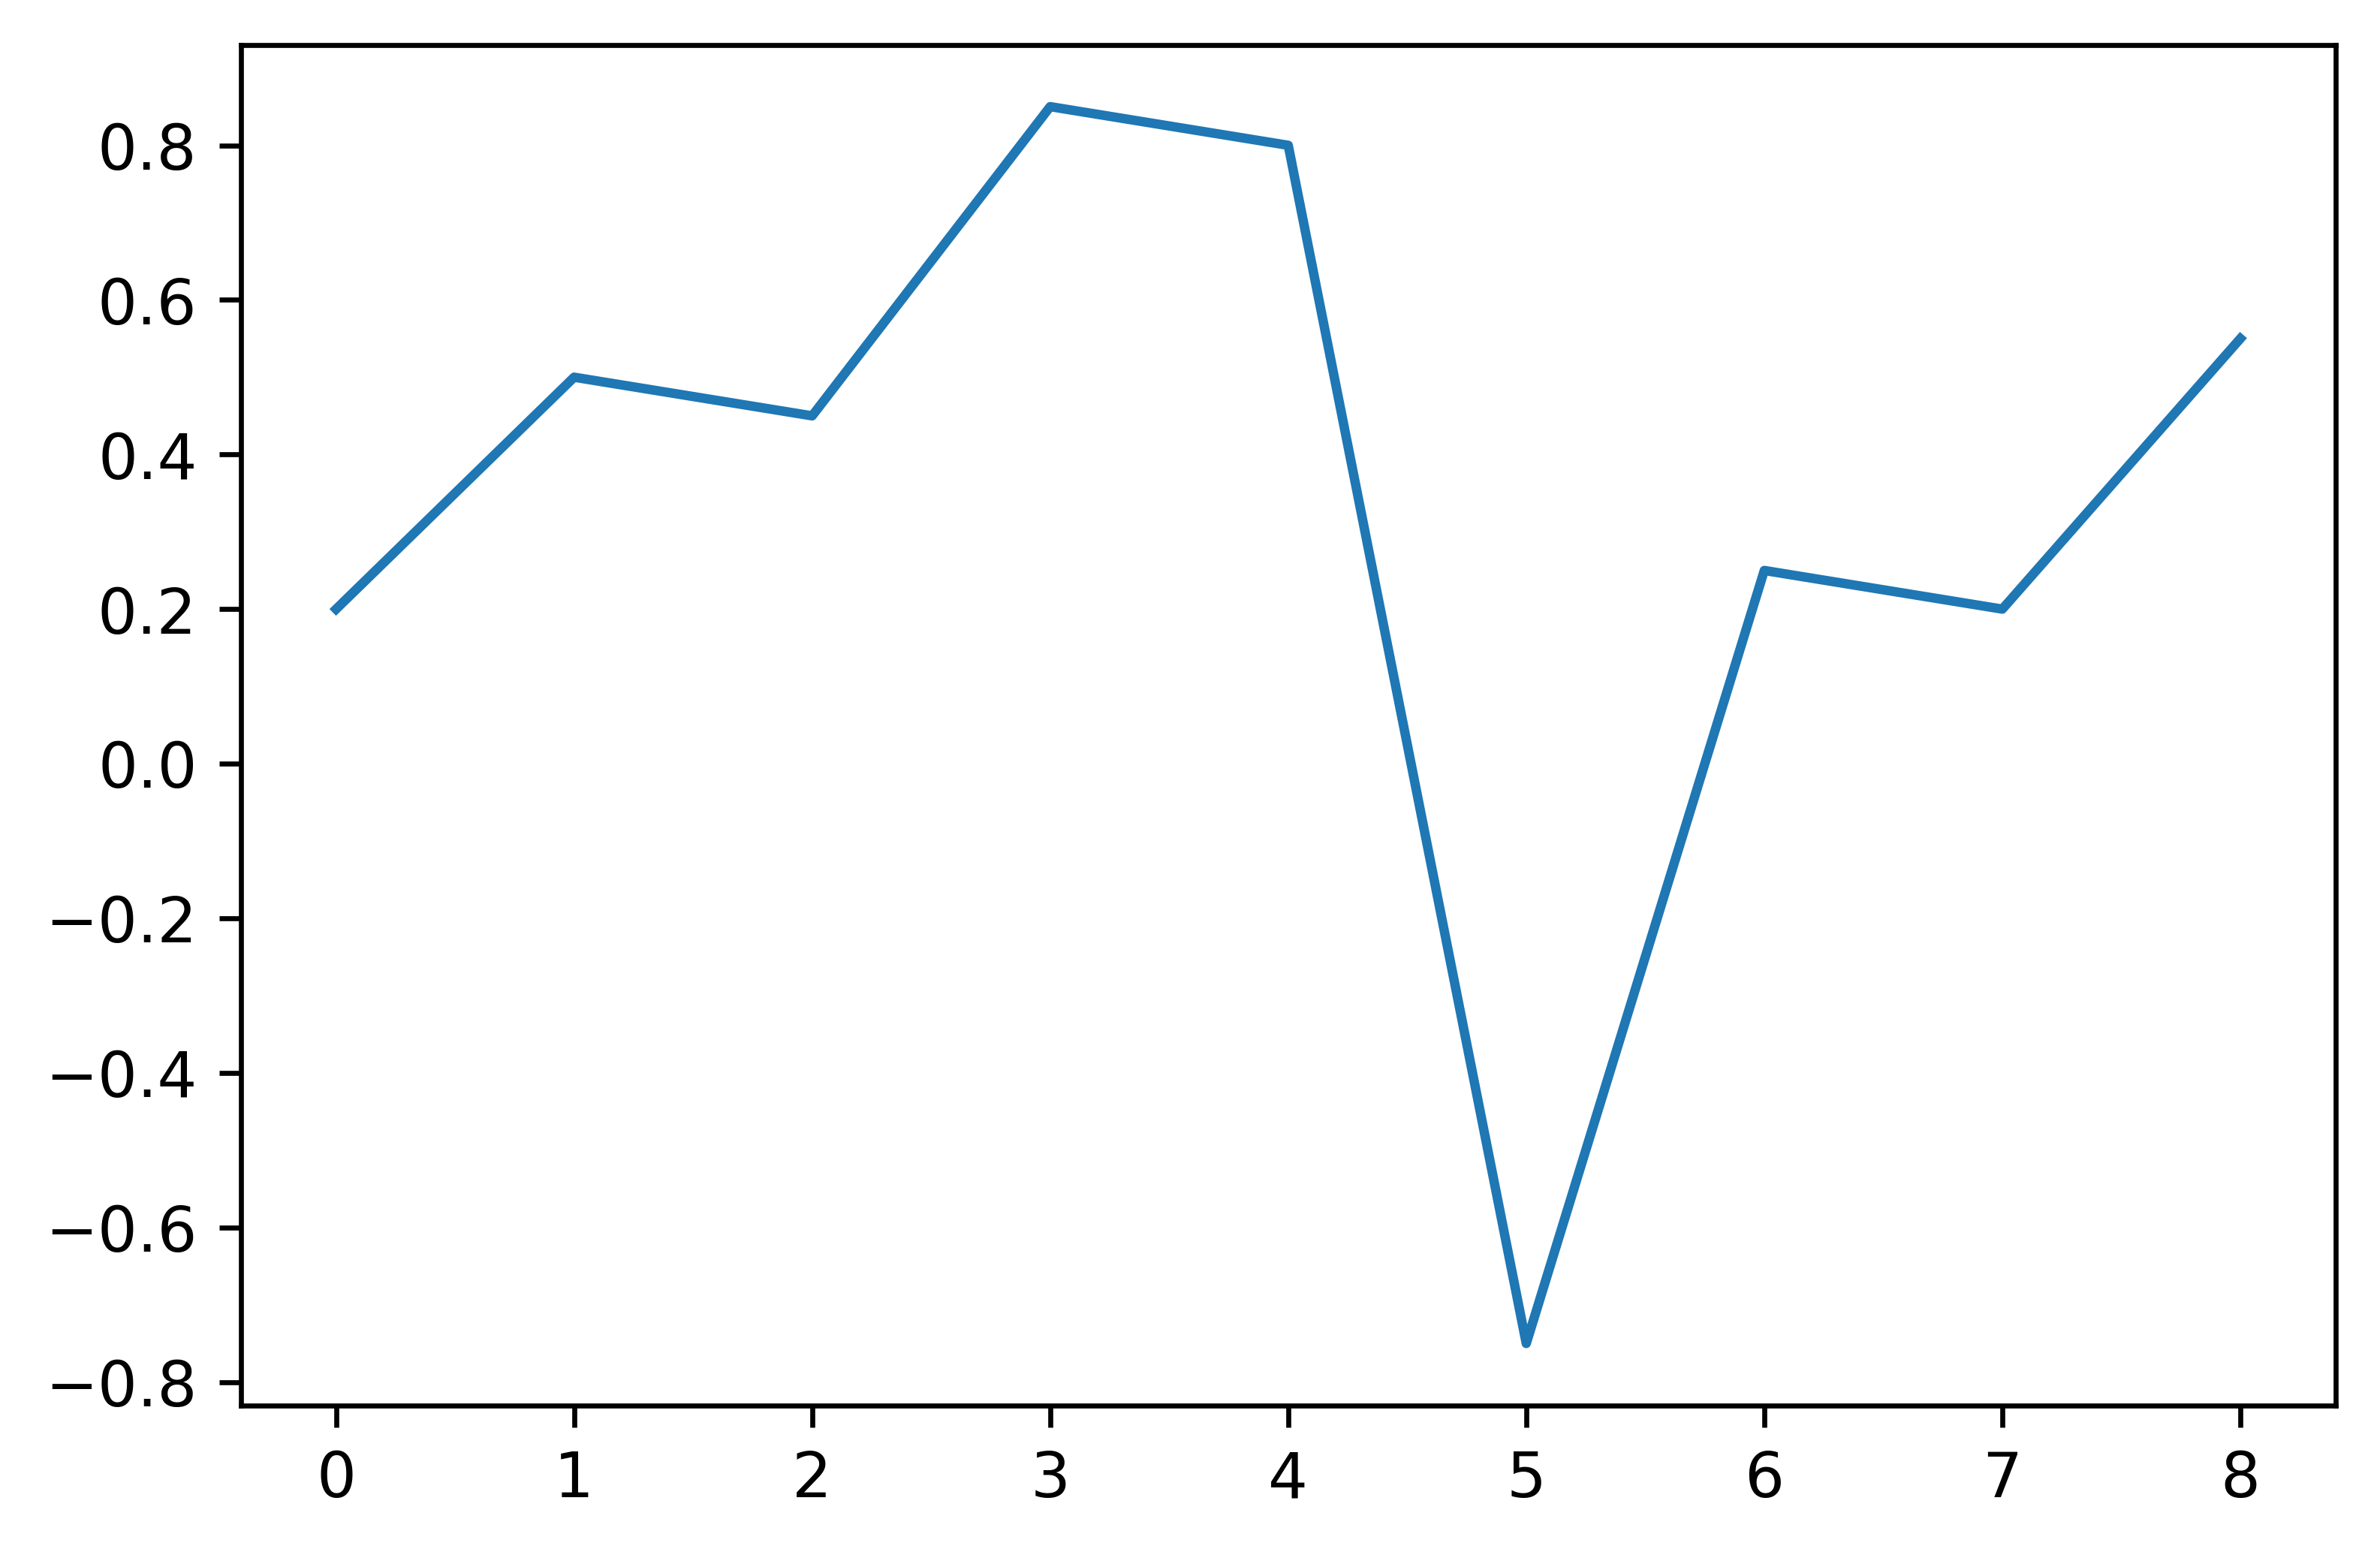
\includegraphics[scale=0.5]{Graphics/guido20118-pattern.png}
	\caption{Patrón usado en \cite{Guido2018} con valores [0.20, 0.50, 0.45, 0.85, 0.80, -0.75, 0.25, 0.20, 0.55].} \label{fig:Guido2018-pattern}
\end{figure}

En esta sección se describe paso a paso la construcción del filtro $q[\cdot]$ para la detección del
patrón $m[\cdot]$ que se muestra en la Figura \ref{fig:Guido2018-pattern}. El método numérico usado para hallar
la solución del sistema de ecuaciones no lineales fue el método de Levenberg-Marquardt.

Según los pasos descritos en la Sección \ref{algoritmo:dst-2}, las ecuaciones del sistema son las siguientes:

\begin{itemize}
	\item \textbf{Paso 1:} La ecuación de la energía unitaria (\ref{eq:unitary-energy}):
		\begin{equation}
			q_0^2 + q_1^2 + q_2^2 + q_3^2 + q_4^2 + q_5^2 + q_6^2 + q_7^2 - 1 = 0.
		\end{equation}
	\item \textbf{Paso 2:} Dos ecuaciones de momentos nulos (\ref{eq:vanishing-moments}):
		\begin{equation}
			q_1 + q_2 + q_3 + q_4 + q_5 + q_6 + q_7  = 0
		\end{equation}
		\begin{equation}
			q_1 + 2q_2 + 3q_3 + 4q_4 + 5q_5 + 6q_6 + 7q_7 = 0
		\end{equation}
	\item \textbf{Paso 3:} Tres ecuaciones para las condiciones de ortogonalidad (\ref{eq:orthogonality}):
		\begin{equation}
			q_0q_2 + q_1q_3 + q_2q_4 + q_3q_5 + q_4q_6 + q_5q_7 = 0
		\end{equation}
		\begin{equation}
			q_0q_4 + q_1q_5 + q_2q_6 + q_3q_7 = 0
		\end{equation}
		\begin{equation}
			q_0q_6 + q_1q_7 = 0
		\end{equation}
	\item \textbf{Paso 4:} Las condiciones de detección (\ref{eq:original-matching-1})(\ref{eq:original-matching-2}): 
		\begin{equation}
			0.2q_0 + 0.5q_1 + 0.45q_2 + 0.85q_3 + 0.8q_4 - 0.75q_5 + 0.25q_6 + 0.2q_7 = 0
		\end{equation}
		\begin{equation}
			0.5q_0 + 0.45q_1 + 0.85q_2 + 0.8q_3 - 0.75q_4 + 0.25q_5 + 0.2q_6 + 0.55q_7 = 0
		\end{equation}
	\item \textbf{Paso 5:} Agrupando todas las ecuaciones se obtiene el sistema de ecuaciones no lineales:
		\begin{equation}\label{eq:system}
			\left\{ \begin{array}{rcl}
						q_0^2 + q_1^2 + q_2^2 + q_3^2 + q_4^2 + q_5^2 + q_6^2 + q_7^2 - 1 = 0 \\
						q_1 + q_2 + q_3 + q_4 + q_5 + q_6 + q_7  = 0 \\
						q_1 + 2q_2 + 3q_3 + 4q_4 + 5q_5 + 6q_6 + 7q_7 = 0 \\
						q_0q_2 + q_1q_3 + q_2q_4 + q_3q_5 + q_4q_6 + q_5q_7 = 0 \\
						q_0q_4 + q_1q_5 + q_2q_6 + q_3q_7 = 0 \\
						q_0q_6 + q_1q_7 = 0 \\
						0.2q_0 + 0.5q_1 + 0.45q_2 + 0.85q_3 + 0.8q_4 - 0.75q_5 + 0.25q_6 + 0.2q_7  = 0\\
						0.5q_0 + 0.45q_1 + 0.85q_2 + 0.8q_3 - 0.75q_4 + 0.25q_5 + 0.2q_6 + 0.55q_7 = 0\\
					\end{array}
				\right.
			\end{equation}
\end{itemize}

Luego de resolver el sistema (\ref{eq:system}) se obtiene como solución el siguiente vector para $q[\cdot]$:

$$
	\begin{array}{lcl}
		q[\cdot] = \{ 0.6847497581435479, 0.22696568380592325, 0.14564494606257186,  \\ 
					-0.6216329207785873, 0.18823424339300499, -0.0553137649474309, \\ 
					-0.05756235031820252, 0.1736641627827206 \}.
	\end{array}
$$

Una vez que se tiene el valor de $q[\cdot]$ se procede a calcular el resto de los filtros:

$$
	\begin{array}{lcl}
		p[\cdot] = \{  -0.17366416278272068, -0.05756235031820252, 0.0553137649474309, \\ 
					0.18823424339300499, 0.6216329207785873, 0.14564494606257186, \\
					-0.22696568380592325, 0.684749758143547\},
	\end{array}
$$

$$
	\begin{array}{lcl}
		\bar p[\cdot] = \{ -0.17366416278272068, 0.6847497581435479, -0.22696568380592325, \\ 
							0.14564494606257186, 0.6216329207785873, 0.18823424339300499, \\ 
							0.0553137649474309, -0.05756235031820252 \},
	\end{array}
$$

$$
	\begin{array}{lcl}
		\bar q[\cdot] = \{ -0.6847497581435479, 0.22696568380592325, -0.14564494606257186,\\
			-0.6216329207785873, -0.18823424339300499, -0.0553137649474309, \\ 
		0.05756235031820252, 0.17366416278272068 \},
	\end{array}
$$

Así es posible realizar la DST-II sobre cualquier señal para detectar la presencia
del patrón $m[\cdot]$. Como paso opcional si se quiere obtener las funciones \textit{major} y \textit{minor}
\textit{shapelets} se procedería a resolver los sistemas formados por las ecuaciones  $\Gamma(x)=\sum_k p_k \Gamma(2N-k)$ y 
$\Theta(x)=\sum_k q_k \Theta(2N-k)$.

Para demostrar el uso de las DST-II en la detección de patrones y formas, el patrón $m[\cdot]$ (Figura \ref{fig:Guido2018-pattern}) 
fue insertado en la señal $s[\cdot]$, dando como resultado la siguiente señal (Figura \ref{fig:example-guido-signal}):

\begin{equation}
	s[x] = \left\{ \begin{array}{rcl}
			\cos{\frac{27\pi x}{8}}\sin{\frac{75\pi x}{8}} & \mbox{si} &  0\leq x \leq 40 \\
			m[x]    &    \mbox{si}     &     41\leq x \leq 49     \\
			\cos{\frac{295\pi x}{32}}\sin{\frac{105\pi x}{32}} & \mbox{si} &  50\leq x \leq 63 \\
					 \end{array}
	\right.
\end{equation}

\begin{figure}
	\centering
	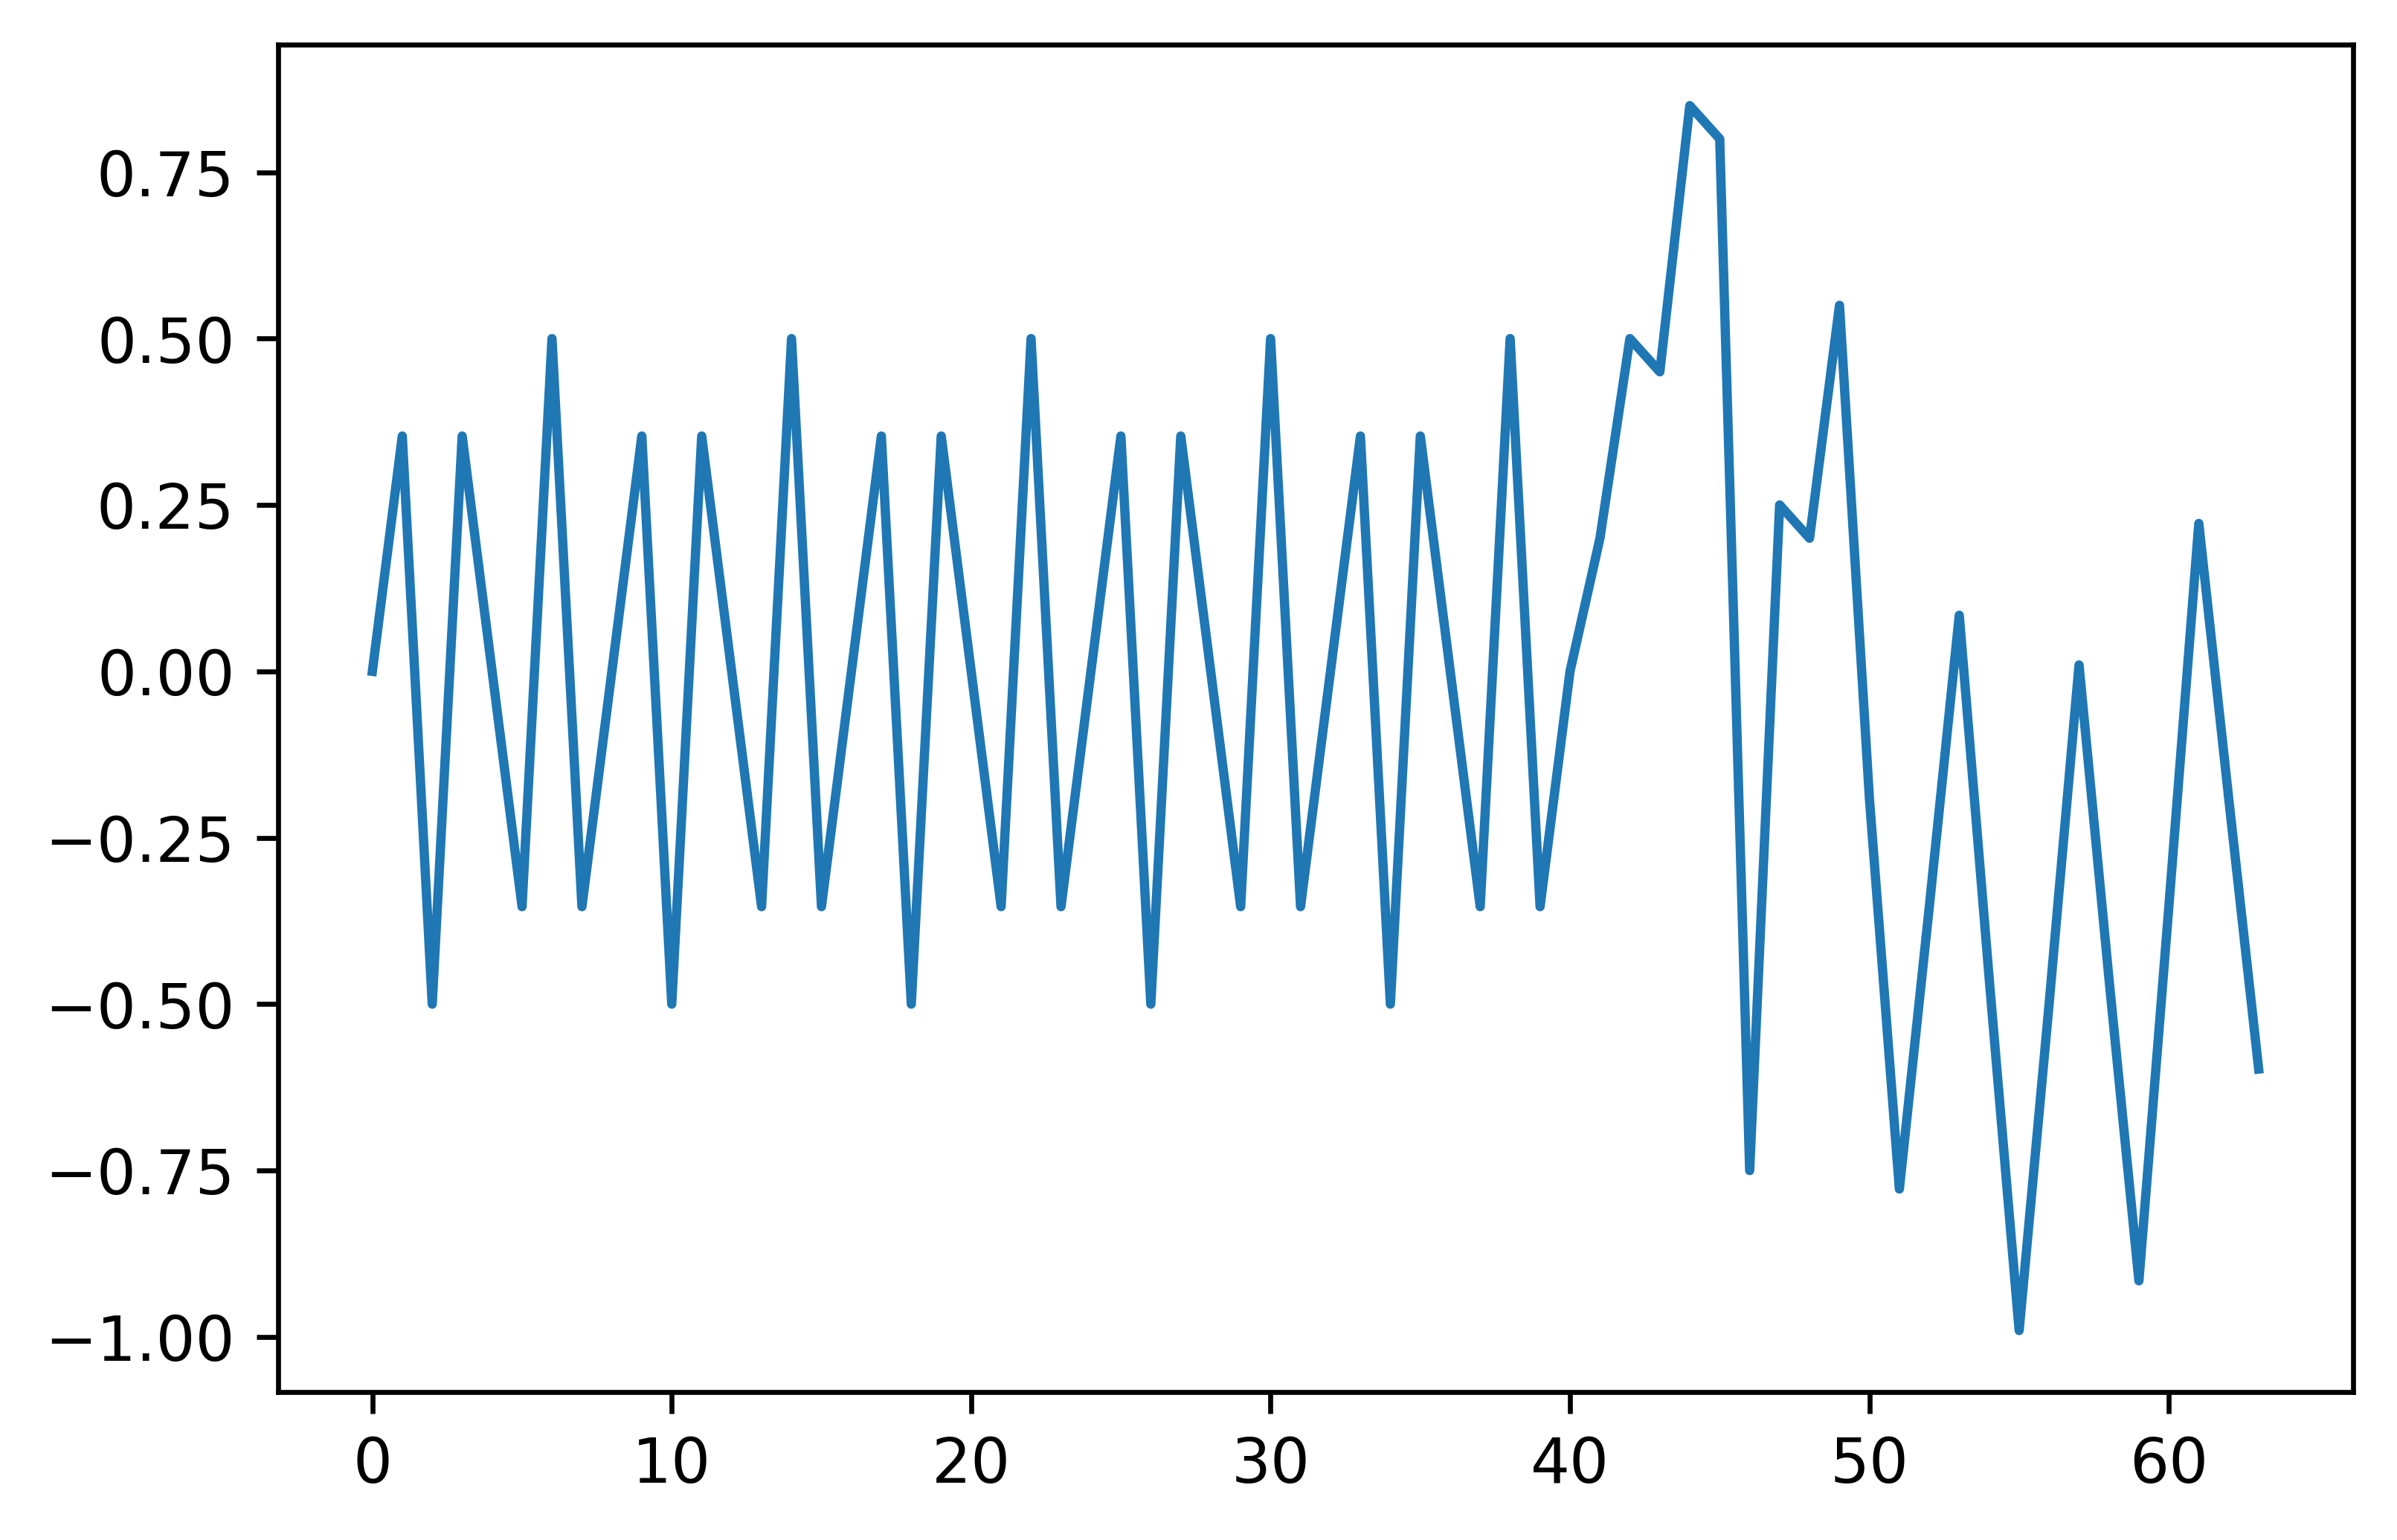
\includegraphics[scale=0.8]{Graphics/example-guido-signal.png}
	\caption{Señal $s$ con patrón $m$ insertado en la posición 41.} \label{fig:example-guido-signal}
\end{figure}

\begin{figure}
	\centering
	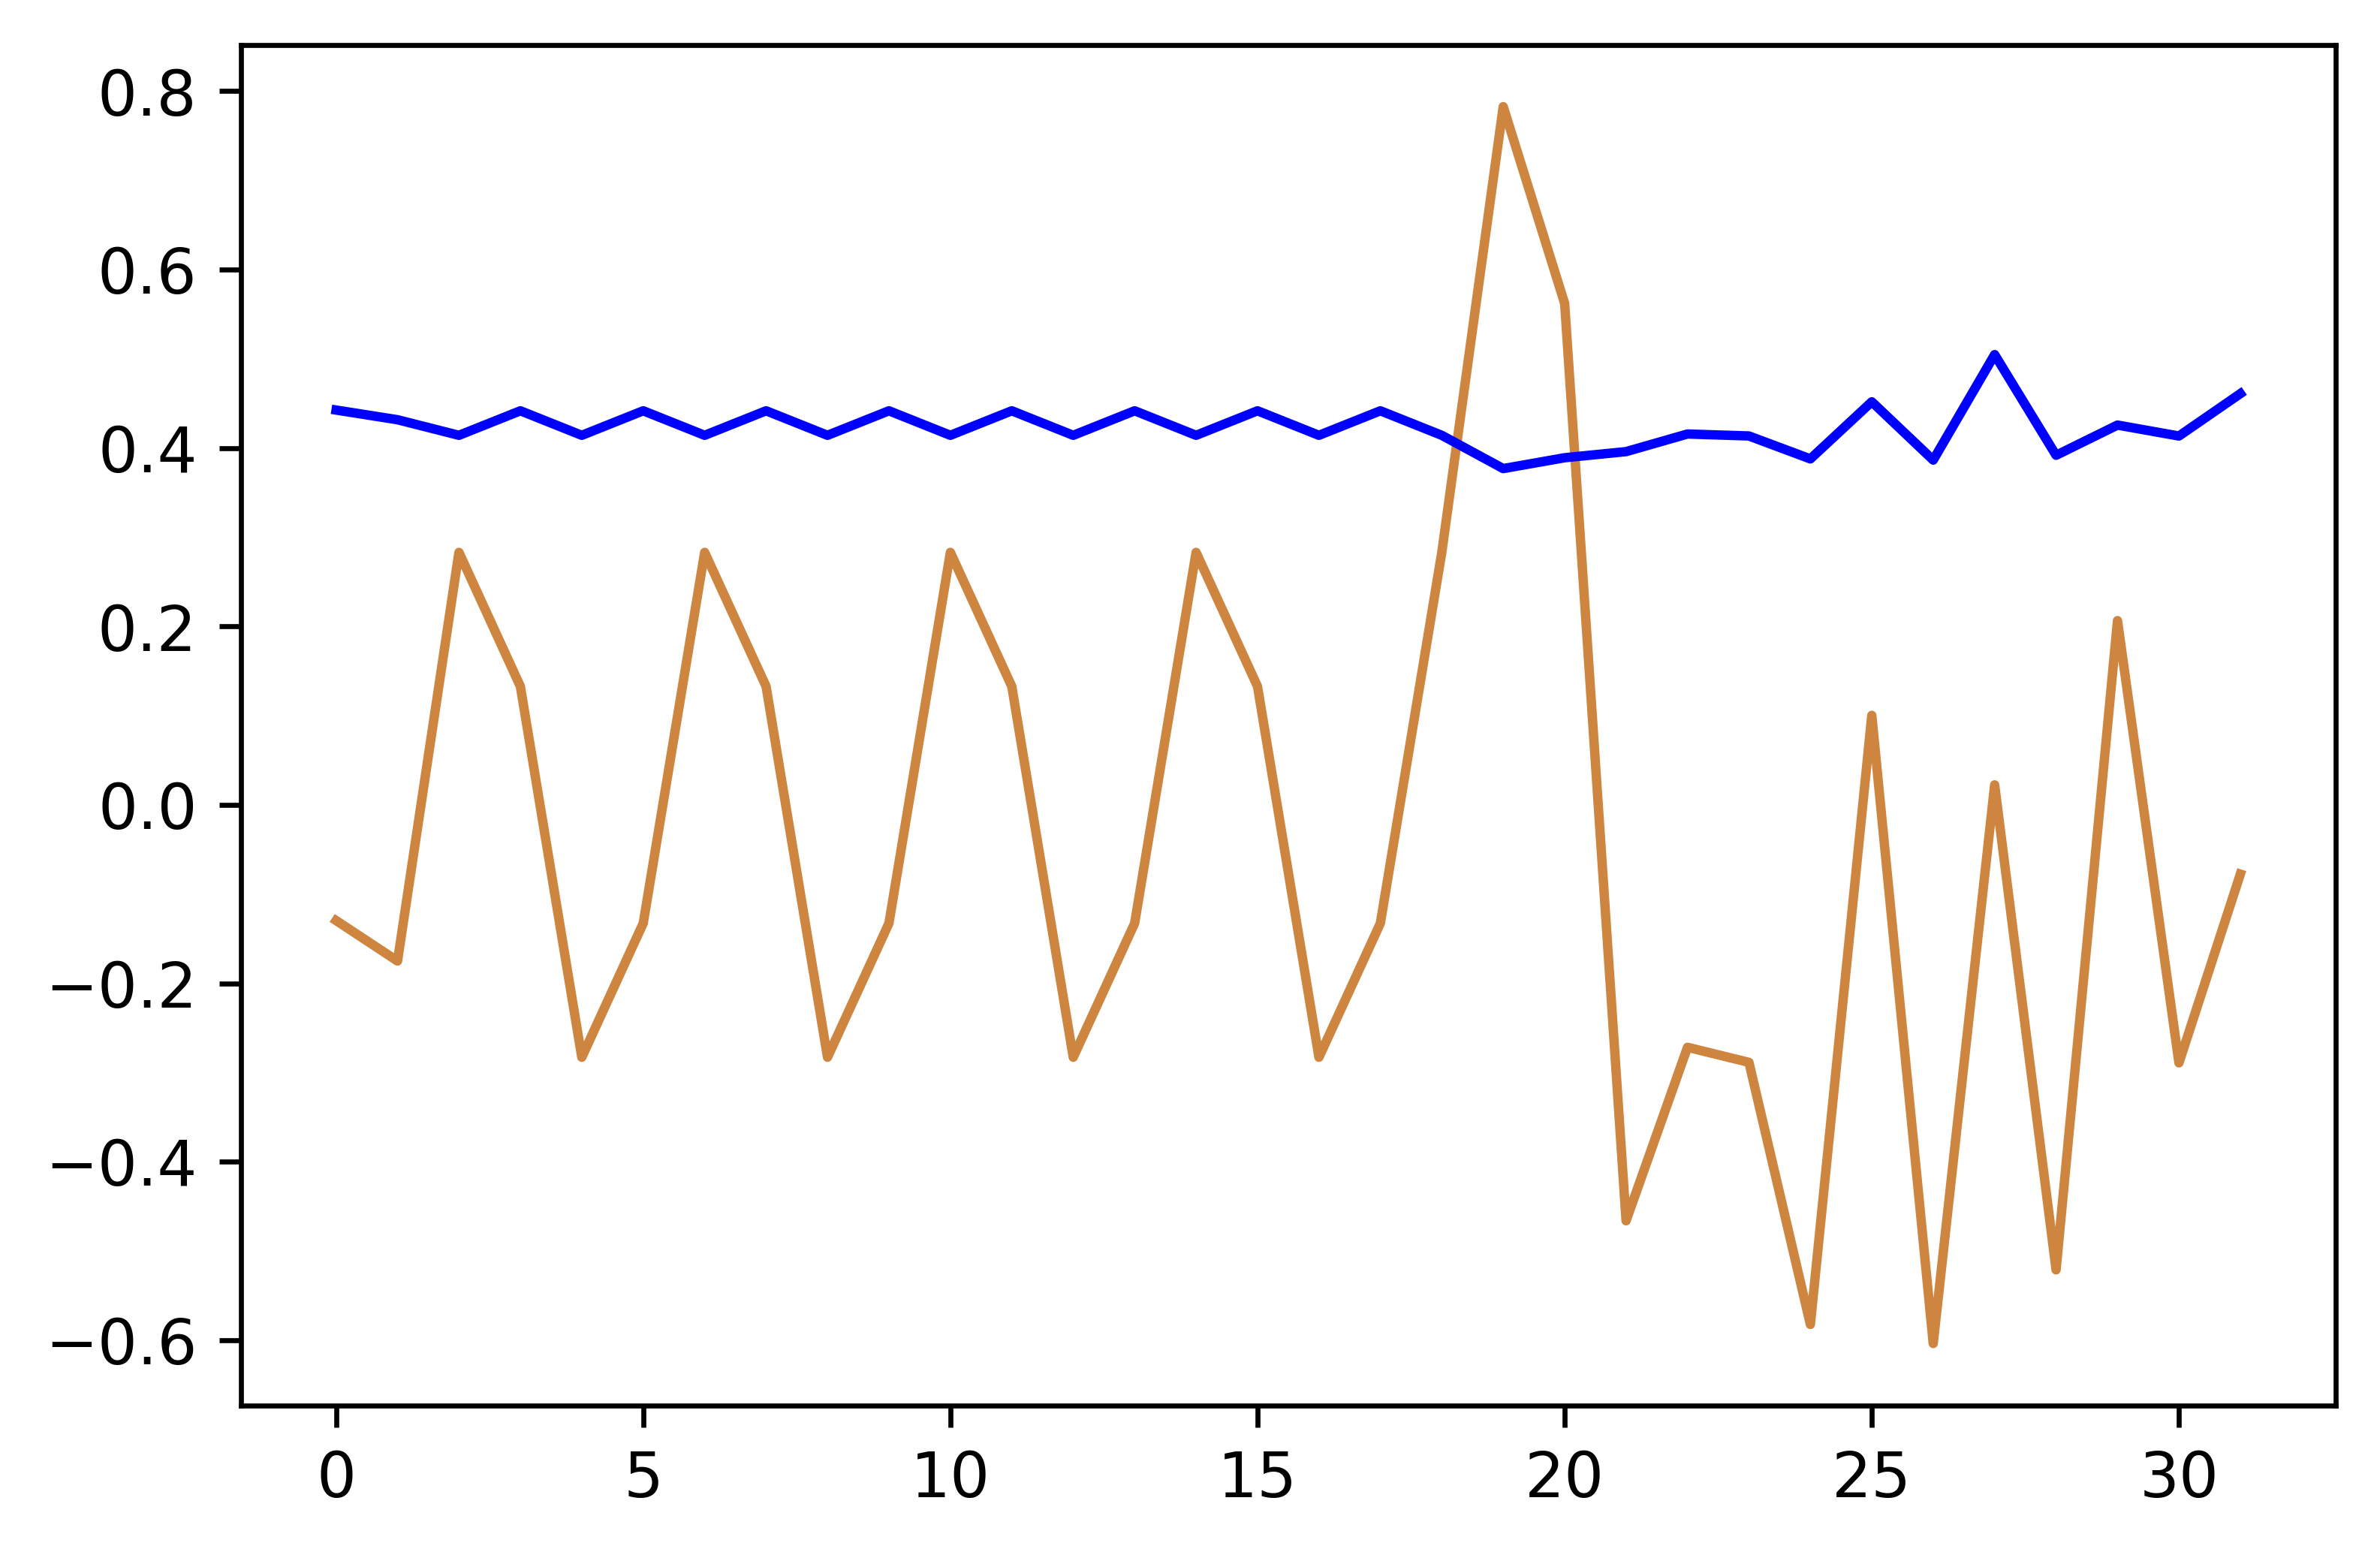
\includegraphics[scale=0.8]{Graphics/example-guido-signal-dst-s-wrong-matching.png}
	\caption{DST-II y medida $\mathbb{S}$.} \label{fig:example-guido-signal-dst-s-wrong-matching}
\end{figure}


La Figura \ref{fig:example-guido-signal-dst-s-wrong-matching} muestra el resultado de la DST-II sobre la señal $s[\cdot]$.
El gráfico color marrón representa la sección \textit{second-rated} del resultado de ls DST-II sobre $s[\cdot]$.
El de color azul corresponde a la medida $\mathbb{S}$ sobre los coeficientes de la \textit{second-rated}. 
Sin embargo, en este gráfico se puede observar que en $\mathbb{S}$ no existe un pico que sobresale del resto del
gráfico, a diferencia de como sucede en el ejemplo de \cite{Guido2018}. De hecho, el punto más alto
se alcanza en el coeficiente número 27, que no corresponde con la ubicación del patrón en la señal 
original. Además, en esta posición $\mathbb{S}=0.50$, lo cual implica que no se detecta el patrón.

\subsection{Reajuste en las condiciones de detección}

La DST-II está diseñada para que las condiciones de detección 
permitan obtener un valor lo más cercano a $0$ cuando se realiza la convolución entre el filtro $q[\cdot]$
y el patrón $m[\cdot]$. Sin embargo, es necesario hacer una modificación a las ecuaciones 
para que esto funcione.

De (\ref{eq:mallat-details}) se tiene que la convolución se hace multiplicando el filtro de atrás hacia adelante 
con la sección de la señal que se está procesando. Por lo que en vez usar las ecuaciones (\ref{eq:original-matching-1})
y (\ref{eq:original-matching-2}) se usan las siguientes:

\begin{equation}\label{eq:matching-1}
	\sum_{k=1}^{N} q_{N-k}m_{k} = 0,
\end{equation}
\begin{equation}\label{eq:matching-2}
	\sum_{k=1}^{N} q_{N-k}m_{k-1} = 0.
\end{equation}

Usando estas nuevas fórmulas, se obtienen las siguientes ecuaciones para el ejemplo del patrón de 
la Figrua \ref{fig:Guido2018-pattern}:

\begin{equation}
	0.2q_0 + 0.25q_1 - 0.75q_2 + 0.8q_3 + 0.85q_4 + 0.45q_5 + 0.5q_6 + 0.2q_7 = 0
\end{equation}
\begin{equation}
	0.55q_0 + 0.2q_1 + 0.25q_2 - 0.75q_3 + 0.8q_4 + 0.85q_5 + 0.45q_6 + 0.5q_7 = 0
\end{equation}

Después de sustituir las ecuaciones de detección anteriores en el sistema (\ref{eq:system}) se resuelve el sistema
de ecuaciones no lineales y se obtiene la siguiente solución:

$$
	\begin{array}{lcl}
		q[\cdot] = \{ 0.8505813325748994, -0.24960592535063272, 0.22199103863909603,\\ 
			0.29414386817594423, -0.10204570231699035, -0.25121801175290576, \\ 
		0.019678016661321896, 0.06705671594416668 \}.
	\end{array}
$$

Luego, a partir de $q$ se obtienen:

$$
	\begin{array}{lcl}
		p[\cdot] = \{ -0.06705671594416668, 0.019678016661321896, 0.25121801175290576,\\ 
			-0.10204570231699035, -0.29414386817594423, 0.22199103863909603, \\ 
			0.24960592535063272, 0.8505813325748994\},
	\end{array}
$$

$$
	\begin{array}{lcl}
		\bar p[\cdot] = \{ -0.06705671594416668, 0.8505813325748994, 0.24960592535063272,\\ 
			0.22199103863909603, -0.29414386817594423, -0.10204570231699035,\\ 
		0.25121801175290576, 0.019678016661321896 \},
	\end{array}
$$

$$
	\begin{array}{lcl}
		\bar q[\cdot] = \{ -0.8505813325748994, -0.24960592535063272, -0.22199103863909603,\\
			0.29414386817594423, 0.10204570231699035, -0.25121801175290576, \\ 
		-0.019678016661321896, 0.06705671594416668 \}.
	\end{array}
$$

\begin{figure} 
	\centering
	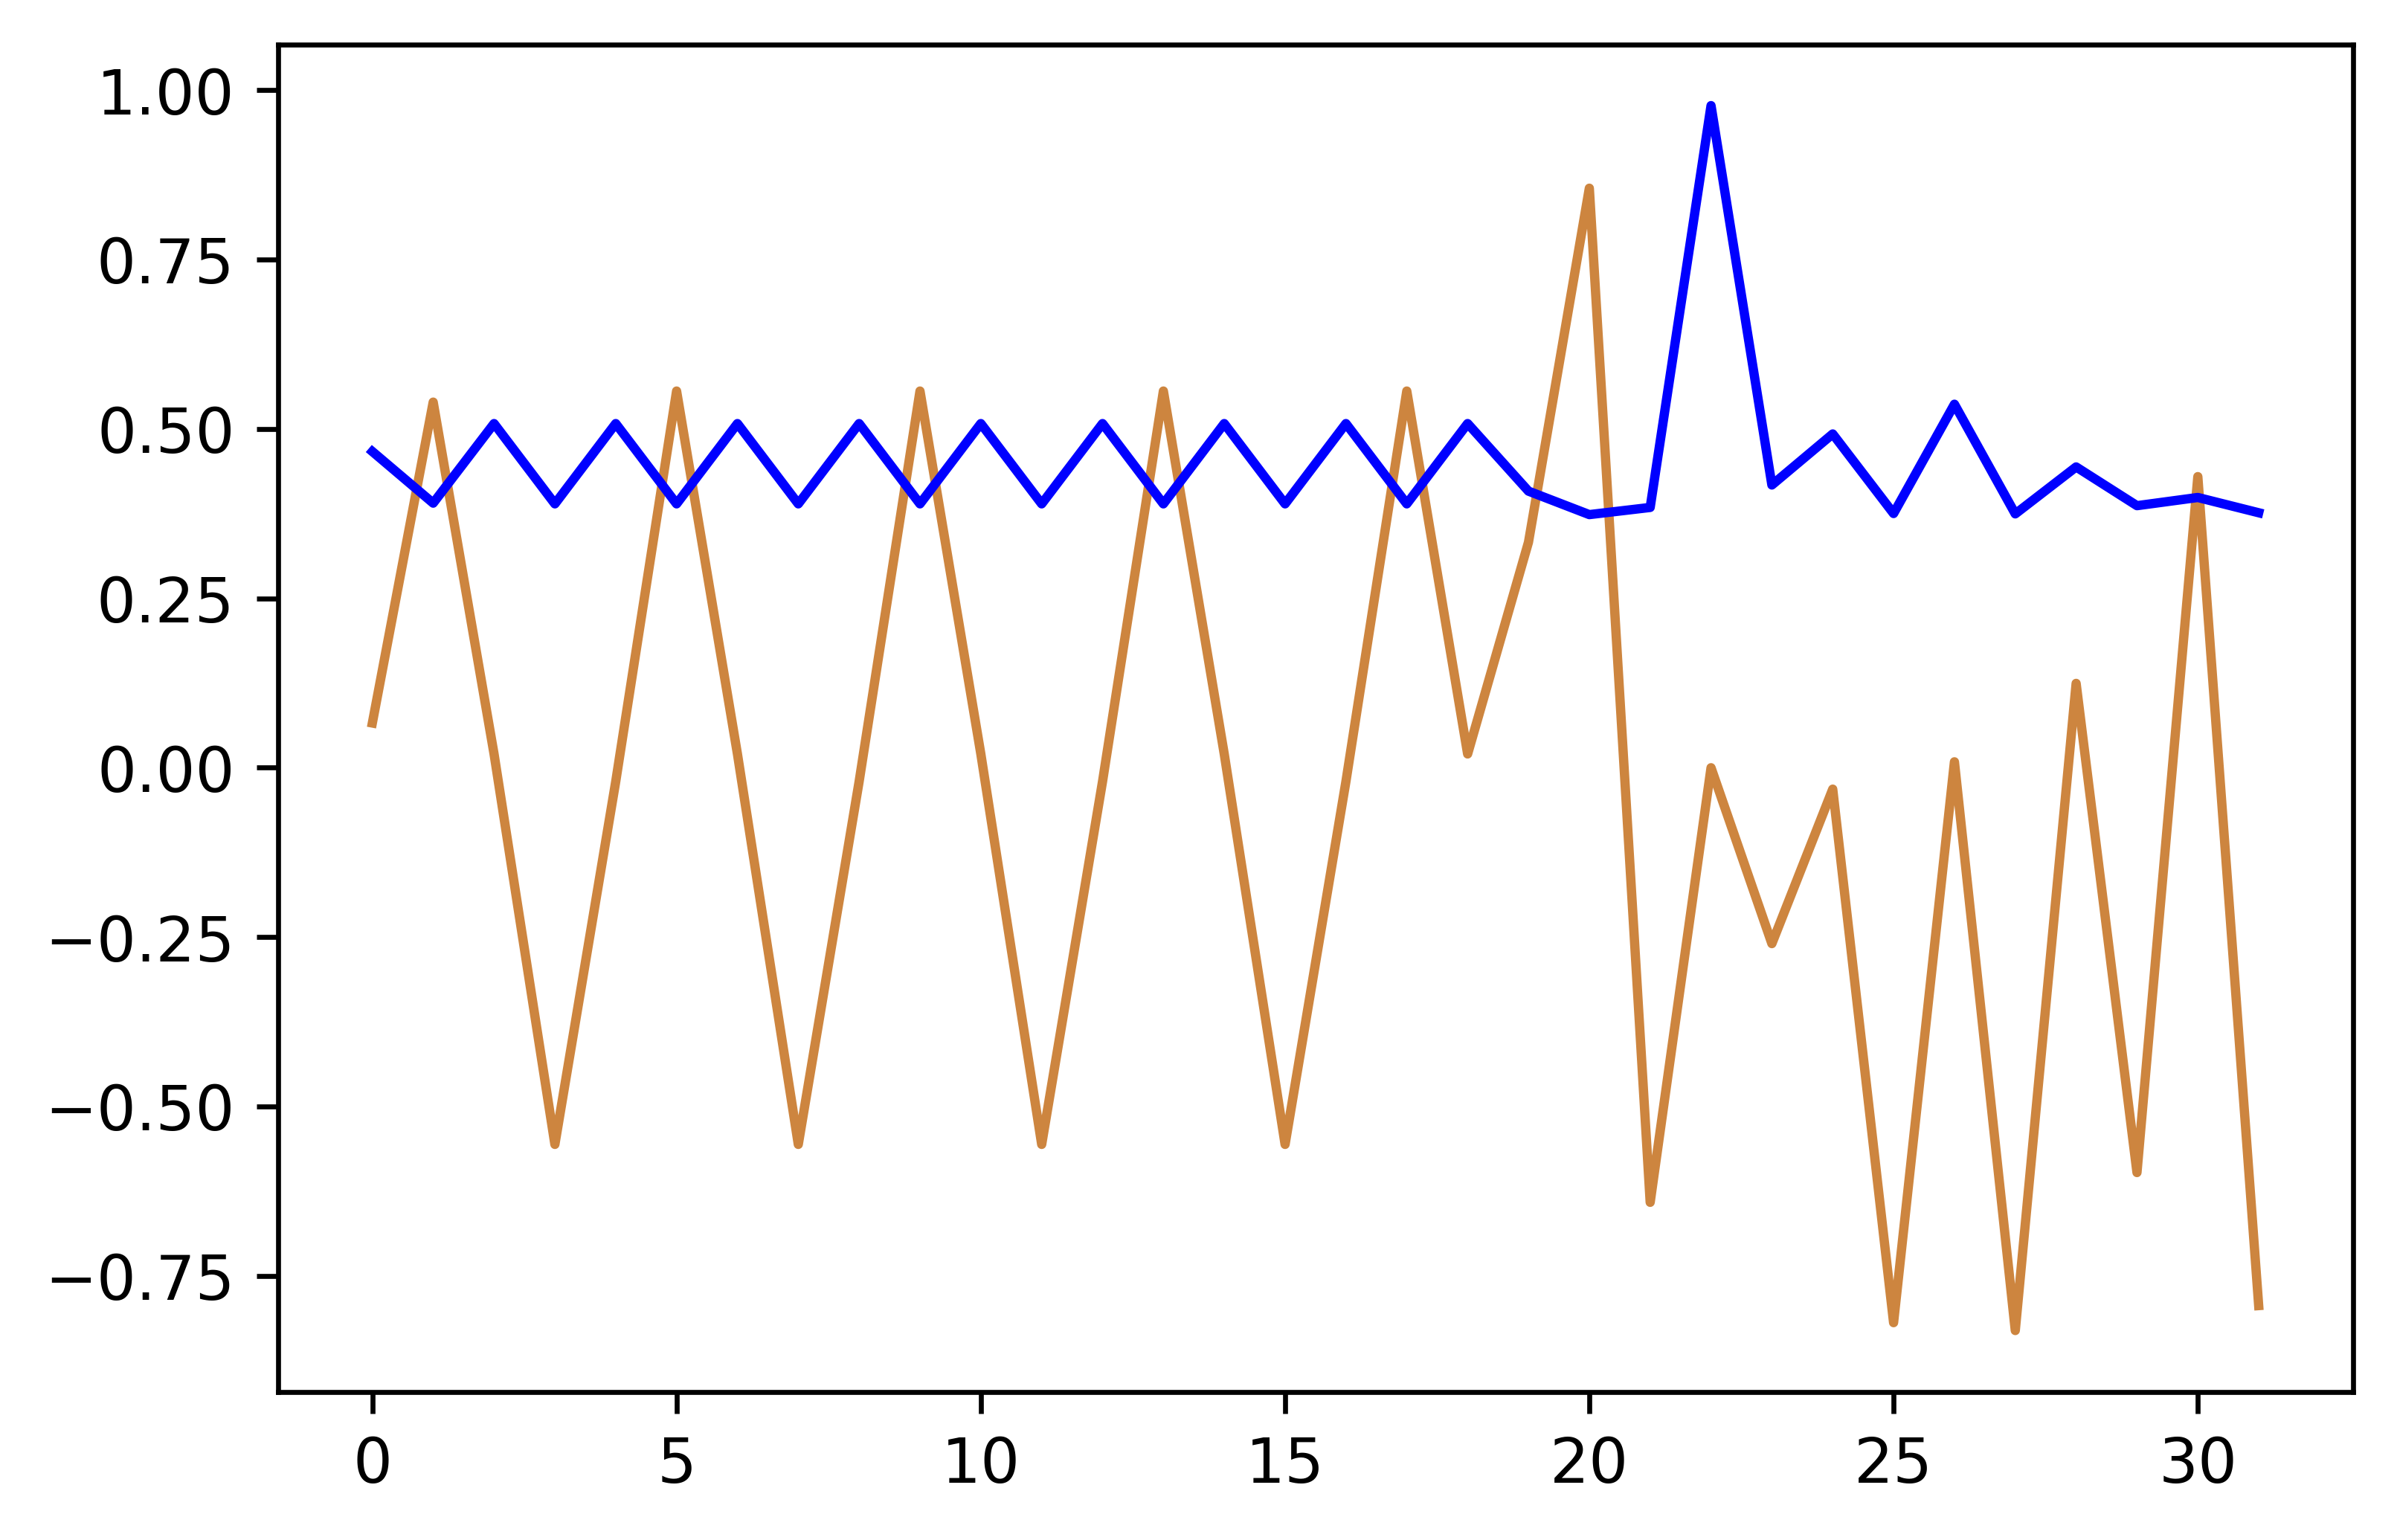
\includegraphics[scale=0.8]{Graphics/example-guido-signal-dst-s.png}
	\caption{DST-II y medida $\mathbb{S}$.} \label{fig:example-guido-signal-dst-s}
\end{figure}

Usando los filtros anteriores se obtiene el resultado mostrado en la Figura \ref{fig:example-guido-signal-dst-s}. 
En este caso, la presencia de $m[\cdot]$ se confirma en la posición $22$ de la DST-II y de $\mathbb{S}$, donde se alcanzan valores
cercanos a $0$ y a $1$, respectivamente ($\mathbb{S}=0.9$). Este coeficiente corresponde a la posición 
$44$ en la señal original. Como se puede apreciar, existe un ligero desplazamiento en la posición donde se detecta $m[\cdot]$,
pero no es de gran tamaño. De hecho, si se toma el coeficiente anterior, la detección es exacta.

\section{Extensión de la DST-II para señales 2D}\label{section:2d}

La DST-II fue diseñada para el caso unidimensional. En este trabajo se busca experimentar sobre las formas en que
este algoritmo se puede extender al caso de señales de bidimensionales. 
En el caso 2D, el patrón $m[\cdot]$ sería en realidad
una matriz $M$ y, por tanto, se tomarían filas o columnas del mismo para construir la shapelet.
La señal $s[\cdot]$ también pasa a ser una matriz, denotada por $X$.
Dado que se está trabajando con imágenes y secciones de las mismas, se va a usar de ahora en adelante la notación
$[A:B,C:D]$ para describir una región o porción de la imagen. $A$ y $B$ representan el intervalo en las filas
comprendidos entre dichos valores. De forma similar, lo hacen $C$ y $D$, pero para las columnas.
A continuación se exponen algunas ideas sobre la extensión de la DST-II para imágenes y la detección de patrones en este tipo de señales.

\subsection{Primera alternativa: DST-II por filas y luego columnas}

La DST-II comparte muchas de las características de la TWD. Ambas transformadas se pueden obtener a través del
algoritmo de Mallat. Por este motivo, una primera idea para extender la DST-II para señales de dos dimensiones
es usar la descomposición no estándar descrita en el epígrafe \ref{section:dwt-2d}.
Como resultado de la misma se obtendrían cuatro componentes. 

Los coeficientes de aproximación no son de interés para la detección. Nótese que la DST-II realizaba la detección en la sección
\textit{second-rated}, que corresponde a los coeficientes de detalles en la TWD. Por tanto, solo se analizará para
la detección las componentes LH, HL y HH.
En este enfoque, sea $X$ la señal de entrada (imagen) con dimensiones $n\times m$, entonces, al realizar el algoritmo de descomposición estándar,
cada uno de los componentes tiene dimensiones $n/2 \times m/2$. Luego, sea $c_{i,j}$ un coeficiente
ubicado en la fila $i$ y la columna de $j$ de cualquiera de las componentes, el mismo corresponde
a la posición $(2i,2j)$ de $X$.

\subsection{Segunda alternativa: DST-II solamente por filas (columnas)}

Dado que el principal objetivo de extender la DST-II para imágenes es aprovechar su capacidad de detección, la cual funciona 
en el caso unidimensional, otra forma de usarla en señales de dos dimensiones es hacer la transformada
por filas o columnas solamente.
Si se usa este enfoque se pueden tomar secciones horizontales y verticales del patrón que se quiere detectar, para 
la construcción de las \textit{shapelets} y obtener información en filas y columnas.

Sea $X$ la imagen de entrada de dimensiones $n\times m$, entonces, si la DST-II se hace por filas se obtiene
como resultado otra imagen de dimensiones $n \times m/2$. De forma análoga si se hace por columnas, se obtiene
una imagen con dimensiones $n/2 \times m$. Nótese que se está asumiendo que se toma solamente la 
\textit{second-rated} de la DST-II. Luego, sea $c_{i,j}$ el coeficiente $j$ de la \textit{second-rated} 
de la DST-II sobre la fila $i$ , si esta última se hace por filas
entonces el coeficiente corresponde a la fila $i$ y la columna $2j$ en $X$. De forma análoga si se hace
la DST-II por columnas, el coeficiente $c_{i,j}$ corresponde a la fila $2i$ y a la columna $j$ en $X$.

\subsection{Tercera alternativa: DST-II usando varias shapelets}

Dado que mientras más \textit{shapelet} construidas a partir de distintas secciones del patrón pueden brindar más información
sobre su localización, entonces se propone como otra alternativa el mismo enfoque anterior, pero construyendo
varias \textit{shapelets} a partir de distintas secciones del patrón que se quiere detectar. Luego, los resultados
de cada una de las transformadas sobre la señal $X$ se promedian. Con esta técnica lo que se busca es lograr definir
el contorno donde se detectan las distintas partes del patrón.


